\section{The AgentFail Framework}
\label{sec:method}

AgentFail instruments a ReAct-style data-science agent with three diagnostic layers: (1) a five-stage taxonomy plus an independent observability label; (2) a propagation-depth analyser; and (3) counterfactual replay for repairability testing. \Cref{fig:framework} summarises the architecture.

\begin{figure}[t]
\centering
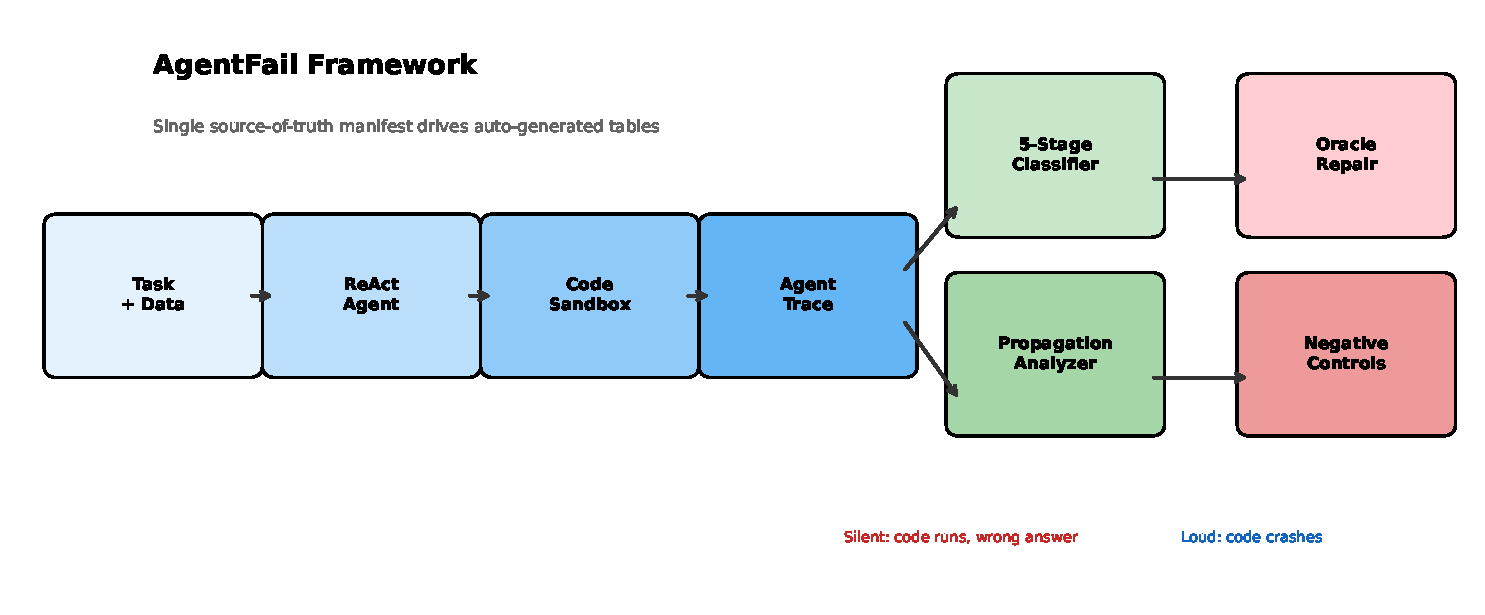
\includegraphics[width=\linewidth]{figures/framework.pdf}
\caption{AgentFail framework. The agent produces a step-by-step trace; the classifier assigns each failure to one of five stages and marks it silent or loud; the propagation analyser computes how far the failure spread; causal replay replaces the originating step with the ground-truth action to test counterfactual dependence.}
\label{fig:framework}
\end{figure}

\subsection{Agent Architecture and Trace Recording}
\label{sec:agent}

We use a ReAct-style agent that interleaves \emph{Thought}, \emph{Action} (a Python code block), and \emph{Observation} (execution output). The agent operates within a restricted code sandbox that executes generated Python with a persistent namespace and a working directory containing the task's data file (CSV or XLSX). We deliberately use a \emph{controlled, minimal} ReAct harness---without few-shot exemplars, code-interpreter scaffolding, or retrieval augmentation---to isolate the diagnostic signal from framework-specific confounds. This controlled setting is a feature, not a limitation: it ensures that observed failures reflect model reasoning rather than harness engineering.

Every step is recorded in an \emph{AgentTrace}, the single source of truth for all downstream diagnosis. Each \texttt{TraceStep} stores the raw LLM output, the parsed thought, the generated code, the execution result (stdout, stderr, exception type, extracted answer), token usage, and a timestamp. Unlike DSBench~\citep{jing2024dsbench}, which retains only a final response, our trace records the full step-by-step trajectory, enabling stage-level localisation and propagation analysis.

\subsection{Five-Stage Failure Taxonomy}
\label{sec:taxonomy}

We decompose every agent failure into one of five stages, defined by \emph{where the error is detectable}, making the categories mutually exclusive:

\begin{itemize}[leftmargin=*,itemsep=2pt]
\item \textbf{Analytical-Plan.} The agent selects the wrong analytical approach: e.g., computing the overall mean when the task requires a per-group sum, or using future data in a time-series analysis (temporal leakage). Often silent.
\item \textbf{Code-Generation.} The agent writes code that embodies a wrong operation: e.g., using \texttt{.count()} where \texttt{.sum()} is needed, selecting the wrong column, or introducing type confusion. Silence varies.
\item \textbf{Runtime (loud).} The generated code raises an exception: runtime errors, type errors, key errors, or sandbox security blocks. The failure is \emph{visible} to the agent, which can observe the traceback and retry.
\item \textbf{Output-Mismatch.} The code executes without error but the agent extracts or reports a result unsupported by the relevant execution output. The mismatch may be silent or explicitly observable (e.g., ``No data found'').
\item \textbf{Answer-Error (silent).} The code runs and produces a result, but the result itself is wrong relative to the ground truth: e.g., a wrong aggregation result or an incomplete analysis. The failure is \emph{invisible} to the agent.
\end{itemize}

Stage and observability answer different questions: stage identifies where the error becomes detectable, whereas \texttt{is\_silent} records whether the trace explicitly exposes failure. Runtime is ordinarily loud and Answer-Error ordinarily silent, but Output-Mismatch and Code-Generation vary. \Cref{tab:taxonomy} lists the hierarchy.

\textbf{Disambiguation rule.} To ensure mutual exclusivity, the classifier assigns the \emph{first} stage at which the error becomes detectable. Consider a task requiring per-group sum where the agent uses \texttt{.count()}: the error is \emph{detectable at code-generation time} (the code uses the wrong operation), so it is classified as Code-Generation, not Answer-Error (where the code uses the correct operation but the data produces a wrong result) or Output-Mismatch (where the code and result are correct but the agent misreports). The key distinction is: Code-Generation means the code itself is wrong; Answer-Error means the code is correct but the answer is wrong due to data issues; Output-Mismatch means the code and result are correct but the agent misreads or hallucinates the final answer. This ordering prevents the ambiguity where a single failure could be assigned to multiple stages.

\begin{table}[t]
\centering
\caption{Five-stage failure taxonomy (v2). Stages are defined by \emph{where the error is detectable}, making them mutually exclusive.}
\label{tab:taxonomy}
\small
\resizebox{\linewidth}{!}{%
\begin{tabular}{@{}lll@{}}
\toprule
Stage & Sub-categories & Observability \\
\midrule
Analytical-Plan & wrong\_operation\_plan, leakage\_plan & often \\
Code-Generation & wrong\_aggregation\_code, wrong\_column, type\_confusion & varies \\
Runtime & runtime\_exception, key\_error, security\_block & No \\
Output-Mismatch & misread\_output, hallucinated\_answer, no\_answer\_printed & varies \\
Answer-Error & wrong\_result, incomplete\_analysis & Yes \\
\bottomrule
\end{tabular}
}
\end{table}

\subsection{Failure Classification}
\label{sec:classifier}

The classifier combines global exception checks, conservative Thought analysis, Thought--Code--\texttt{gt\_path} consistency rules, whole-trace output interpretation, and explicit failure-message detection. Code-Generation rules cover wrong aggregation, wrong dynamic column selection, omitted implementation, and computed-but-unprinted answers. Because reference paths are inputs, this classifier is oracle-assisted rather than deployment-ready. On the final 150-trace human gold set it achieves 91.3\% accuracy (95\% bootstrap CI [86.7, 95.3]) and 90.3\% macro-F1 over the four observed classes; observability accuracy is 99.3\%. Code-Generation precision and recall are both 91.7\%.

\subsection{Propagation Depth}
\label{sec:propagation}

Once a failure originates at step $i$, it may propagate to later steps. We define \emph{propagation depth} as the number of steps from the originating failure to the step where it is detected (or to the trace end if never detected). Loud failures have depth 0 (immediately visible); silent failures can have depth $\geq 1$, meaning the agent continues building on a wrong intermediate result. A propagation depth $\geq 2$ indicates a \emph{long-horizon} failure spread, the most dangerous regime because it wastes the most tokens and is hardest to recover from. Across all 3{,}940 failures, the average propagation depth is 0.30 steps; 88.6\% are detected immediately (depth 0), while 6.9\% propagate to depth $\geq 2$ (see \Cref{tab:propagation} in \Cref{app:datacard}).

\subsection{Oracle-Guided Repair}
\label{sec:causal}

To test whether a failed trace is \emph{repairable}, we adapt the counterfactual principle~\citep{shah2026causal} to the data-science setting. Given a trace that failed, we synthesise a \emph{counterfactual} version of the originating step: the canonical ground-truth code derived from the task's reference solution path. We then replay execution from that point in a fresh sandbox. If the replayed trace now produces the correct answer, the failure was repairable; if the replay still fails, the failure has a deeper root cause.

Formally, let $T = (s_1, \dots, s_n)$ be a failed trace and $s_k$ the classified originating step. Let $s_k^*$ be the ground-truth action for step $k$. We construct the counterfactual trace $T' = (s_1, \dots, s_{k-1}, s_k^*, \dots)$ and execute it. The repair is successful iff $T'$ yields the correct answer. The \emph{oracle repair rate} is the proportion of failed traces for which repair succeeds.

\textbf{Negative control.} A no-op control runs the ground-truth code independently without any step replacement. If the oracle repair rate matches the no-op rate (as we observe, \Cref{sec:disc-negative-control}), the oracle rate measures only whether the ground-truth code produces the correct answer, not step-level causality. We therefore report oracle repair as an upper bound on reparability.

\subsection{Diagnostic Metrics}
\label{sec:metrics}

We report three layers of metrics: \textbf{Layer 1 (task-level):} success rate (SR), code-execution success rate. \textbf{Layer 2 (failure-diagnostic):} silent-failure rate (SFR = proportion of failures that are silent), stage distribution, propagation depth, recovery rate, and oracle repair rate. \textbf{Layer 3 (token-economic):} tokens-per-success and cost-per-success, addressing the under-reporting of cost identified by~\citet{moghadasi2026what}. Verifier comparisons use the McNemar test ($b$, $c$, $\chi^2$ $p$-value).
